% Вопросы членов диссертационного совета и ответы на них.
% Источник: SUPPLEMENTARY/Ответы на вопросы члены диссовета.docx

\section{Ответы на вопросы членов диссертационного совета}

% #1 --- член совета, #2 --- номер вопроса, #3 --- текст вопроса
\newcommand{\qaQuestion}[3]{%
\begin{frame}[noframenumbering]{Вопрос #2. #1}
    \vfill
    \begin{block}{}
        \small #3
    \end{block}
    \vfill
\end{frame}}

% Слайд-заглушка для ещё не подготовленного ответа
\newcommand{\qaTodo}{%
    \vfill
    \centering
    {\Large\color{red}[Ответ дописать]}
    \vfill}

\begin{frame}[plain,noframenumbering]
    \centering
    \vfill
    {\LARGE\color{MIPTBlue}\textbf{Ответы на вопросы членов\\[0.2em]
    диссертационного совета}}
    \vfill
\end{frame}

% ---------------------------------------------------------------------------
% Райгородский А.М.
% ---------------------------------------------------------------------------

\qaQuestion{Райгородский А.М.}{1}{%
    В диссертации предложены методы SPOWL, SG-Safe и ITES, использующие разные
    механизмы обеспечения безопасности. Какие свойства задачи определяют выбор
    между этими подходами? В каких случаях достаточно оценки долгосрочного
    риска, а в каких требуется использование иерархической структуры и
    промежуточных подцелей?}

\begin{frame}[noframenumbering]{Ответ на вопрос 1. Райгородский А.М.}
    \small
    Выбор метода определяется прежде всего горизонтом задачи и разреженностью
    вознаграждения.

    \vspace{0.6em}
    \renewcommand{\arraystretch}{1.35}
    \begin{tabular}{@{}>{\raggedright\arraybackslash}p{0.32\linewidth}>{\raggedright\arraybackslash}p{0.64\linewidth}@{}}
        \toprule
        \textbf{Свойства задачи} & \textbf{Метод} \\
        \midrule
        Короткий горизонт, плотное (евклидово) вознаграждение
            & \textbf{SPOWL}: модель мира и оценка долгосрочного риска,
              лучшие результаты на Safety Gym \\
        Большой горизонт, разреженное вознаграждение; жёсткие ограничения
        по памяти и скорости инференса
            & \textbf{SG-Safe}: подцели снимают чрезмерную консервативность
              безопасной стратегии (робот в лабиринте); генератор подцелей
              нужен только при обучении \\
        Нужно контролировать безопасность и выбора подцелей, и их достижения
            & \textbf{ITES}: безопасность на обоих уровнях иерархии; подходит
              для манипуляции (подойти к объекту, сдвинуть его в нужном
              направлении) \\
        \bottomrule
    \end{tabular}
\end{frame}

\qaQuestion{Райгородский А.М.}{2}{%
    Как увеличение размерности пространства состояний и действий и общей
    сложности среды может повлиять на эффективность предложенных методов? Какие
    компоненты SPOWL, SG-Safe и ITES в первую очередь могут стать
    ограничивающими при переходе к более сложным задачам?}

\begin{frame}[noframenumbering]{Ответ на вопрос 2. Райгородский А.М.}
    \begin{itemize}
        \item \textbf{ITES:} верхний уровень опирается на дискретизированную
              карту пространства целей $(x,y)$ (сеть смежности). С ростом
              размера среды и размерности пространства целей эта карта
              растёт; отображение состояния в пространство целей задаётся
              вручную.
        \item \textbf{SPOWL, SG-Safe, ITES} сейчас работают с векторными
              наблюдениями и не работают с визуальными наблюдениями и
              языковыми командами.
        \item Для более сложных сред потребуется добавить энкодеры
              наблюдений (изображения, текст) и обучать модели мира и штрафов
              в их латентном пространстве.
    \end{itemize}
\end{frame}

\qaQuestion{Райгородский А.М.}{3}{%
    Методы SG-Safe и ITES ориентированы прежде всего на задачи с большим
    горизонтом и разреженным вознаграждением. Как изменится их преимущество по
    сравнению с обычными методами безопасного обучения с подкреплением, если
    задача имеет короткий горизонт или более плотный сигнал вознаграждения? В
    каких случаях использование иерархической структуры может оказаться
    избыточным?}

\begin{frame}[noframenumbering]{Ответ на вопрос 3. Райгородский А.М.}
    \begin{itemize}
        \item При коротком горизонте и плотном вознаграждении (например, за
              приближение к цели) одноуровневая стратегия получает достаточно
              информативный сигнал и решает задачу без подцелей. Здесь
              иерархия может оказаться избыточной.
        \item Однако плотное вознаграждение не всегда решает проблему
              исследования. В лабиринте евклидово расстояние до цели ведёт
              агента к стене, за которой находится цель: чтобы её достичь,
              нужно сначала двигаться в противоположную сторону, а при таком
              вознаграждении это невыгодно.
        \item В таких задачах промежуточные подцели полезнее обычного
              reward shaping.
    \end{itemize}
\end{frame}

% ---------------------------------------------------------------------------
% Гаврилов Д.А.
% ---------------------------------------------------------------------------

\qaQuestion{Гаврилов Д.А.}{1}{%
    В методе SPOWL для оценки будущих накопленных штрафов используется ансамбль
    функций оценки. Как способ агрегации ансамбля влияет на баланс между
    недооценкой риска и чрезмерно консервативным поведением агента? Почему в
    работе выбран используемый способ агрегации?}

\begin{frame}[noframenumbering,shrink=5]{Ответ на вопрос 1. Гаврилов Д.А.}
    \small
    Исследованы три способа агрегации ансамбля $\{\hat{Q}^c_j\}_{j=1}^{N}$:
    \begin{itemize}
        \item \textbf{минимум} --- самая оптимистичная оценка риска: агент
              активнее исследует, но если хотя бы один критик недооценивает
              штрафы, планировщик выбирает небезопасную траекторию; итоговый
              cost заметно выше;
        \item \textbf{максимум} --- самая консервативная оценка: агент
              отказывается и от полезных действий и не учится решать задачу;
        \item \textbf{среднее} (SPOWL) --- наиболее устойчивый баланс между
              вознаграждением и безопасностью (рис.~2.4 диссертации).
    \end{itemize}
    \centering
    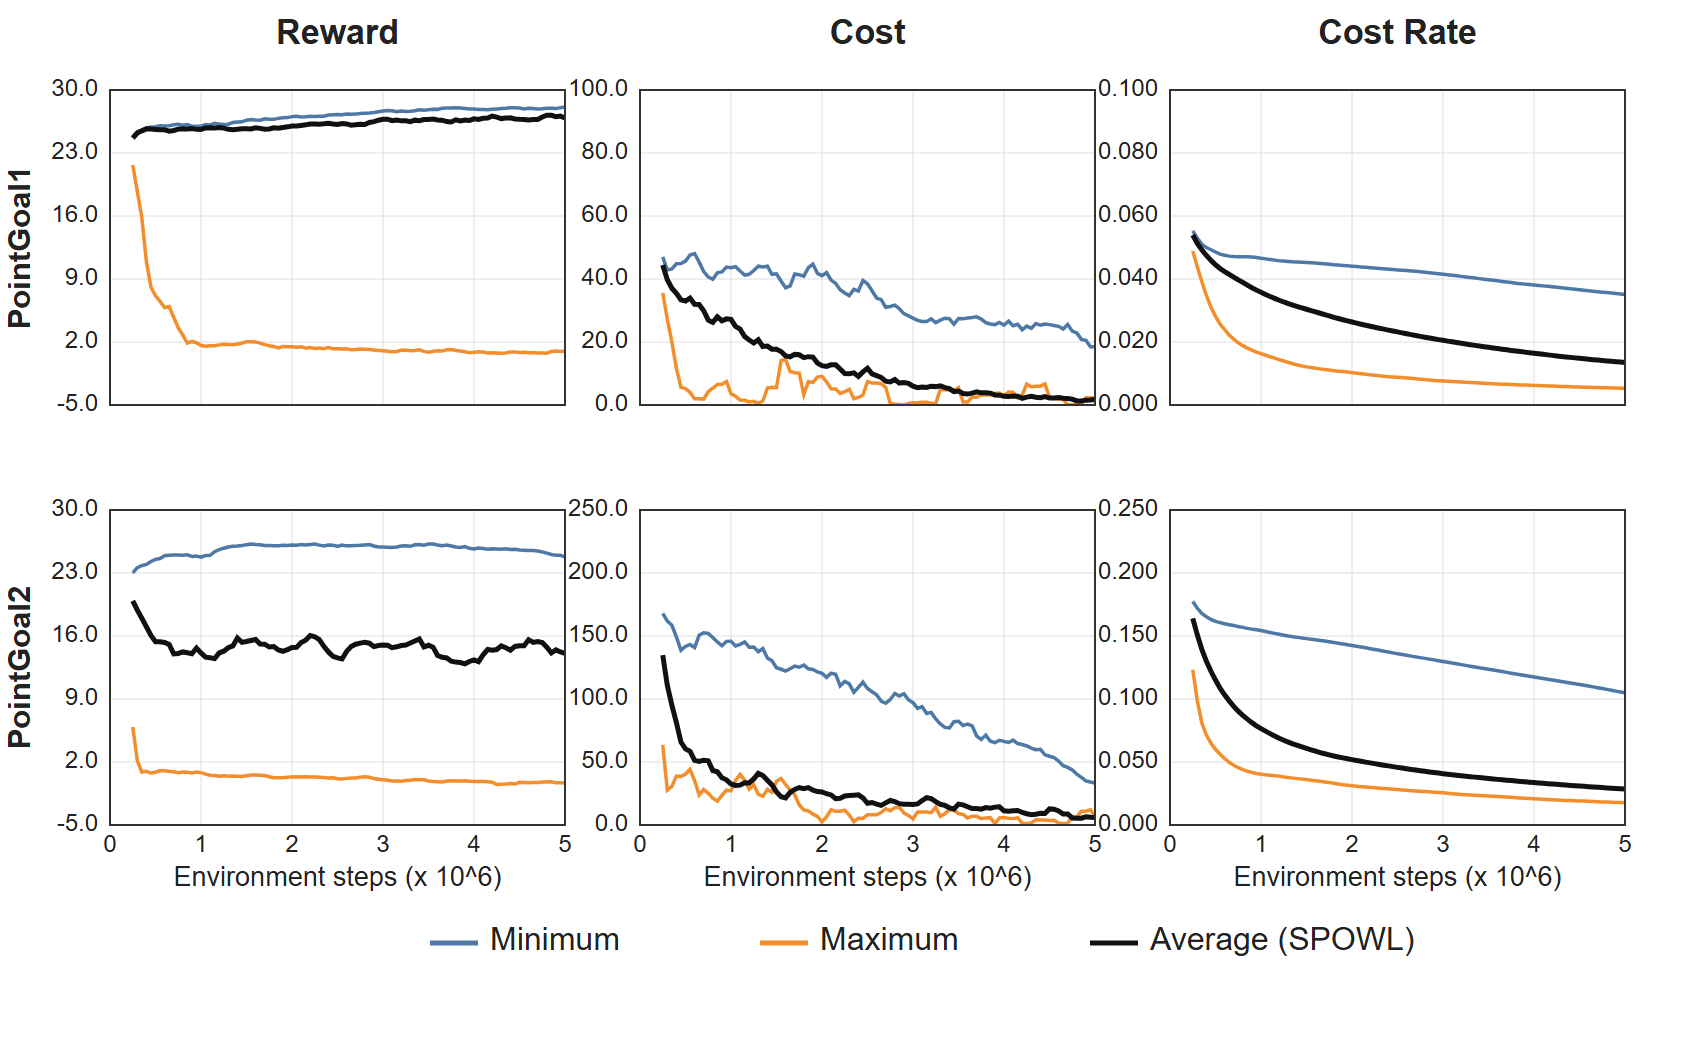
\includegraphics[height=0.47\textheight]{qa/qa_spowl_aggregation}
\end{frame}

\qaQuestion{Гаврилов Д.А.}{2}{%
    В постановке CMDP безопасность задаётся ограничением на ожидаемый
    накопленный штраф. Как можно расширить предложенные методы на
    робототехнические задачи, где часть ограничений должна выполняться на
    каждом шаге, например ограничения на скорость, ускорение или управляющее
    воздействие?}

\begin{frame}[noframenumbering,shrink=5]{Ответ на вопрос 2. Гаврилов Д.А.}
    \small
    \begin{itemize}
        \item \textbf{Безопасная итоговая стратегия:} адаптивно уменьшать
              бюджет штрафов $d$ до нуля в ходе обучения.
        \item \textbf{Безопасность каждого действия во время обучения:} нужна
              априорная информация --- модель объекта управления и явный вид
              функции штрафов. Тогда применимы методы control barrier
              functions и shielding:
    \end{itemize}
    \vspace{-0.3em}
    \begin{columns}[T,onlytextwidth]
        \begin{column}{0.48\textwidth}
            \begin{block}{Модель объекта управления}
                \[
                    \dot{x} = f(x) + g(x)\,u
                \]
            \end{block}
        \end{column}
        \begin{column}{0.48\textwidth}
            \begin{block}{Барьерная функция}
                \[
                    \mathcal{C} = \{x : h(x) \ge 0\},
                \]
                \[
                    \sup_{u \in U}\big[\nabla h(x)\,(f(x) + g(x)u)\big]
                    \ge -\alpha\big(h(x)\big)
                \]
            \end{block}
        \end{column}
    \end{columns}
    \vspace{0.3em}
    \begin{itemize}
        \item Ограничение допустимого множества состояний ещё сильнее сжимает
              исследование, поэтому предложенные в диссертации механизмы
              (подцели, оценка долгосрочного риска) становятся ещё более
              актуальными.
    \end{itemize}
\end{frame}

\qaQuestion{Гаврилов Д.А.}{3}{%
    В SG-Safe генератор промежуточных подцелей используется только во время
    обучения и не входит в контур исполнения. Каким образом информация от
    подцелей переносится в итоговую безопасную стратегию, так что после
    удаления генератора сохраняется улучшенная способность стратегии достигать
    удалённых целей с соблюдением ограничений безопасности?}

\begin{frame}[noframenumbering]{Ответ на вопрос 3. Гаврилов Д.А.}
    \begin{itemize}
        \item Информация сохраняется непосредственно в весах нейронной сети
              стратегии.
        \item Подцели служат дополнительным обучающим сигналом. По сути это
              аналог обучения сложному поведению через reward engineering или
              curriculum-фазы (например, беспилотник, который учится
              парковаться).
        \item Ограничение: сложность итогового поведения ограничена одной
              стратегией над низкоуровневыми действиями, поэтому в более
              сложных задачах манипуляции такой подход, скорее всего, будет
              недостаточен.
    \end{itemize}
\end{frame}

% ---------------------------------------------------------------------------
% Котенко И.В.
% ---------------------------------------------------------------------------

\qaQuestion{Котенко И.В.}{1}{%
    В диссертации безопасность в основном рассматривается через функцию штрафа
    и допустимый бюджет нарушений. Как могут быть расширены предложенные методы
    на случай нескольких независимых ограничений безопасности, например
    ограничений на столкновения, скорость и попадание в опасные области, если
    для каждого из них необходимо контролировать собственный допустимый
    уровень риска?}

\begin{frame}[noframenumbering]{Ответ на вопрос 1. Котенко И.В.}
    \begin{itemize}
        \item Методы на основе функции Лагранжа естественно обобщаются на
              несколько ограничений: каждому виду нарушений соответствует свой
              сигнал штрафа $c_i$ (превышение скорости, приближение к стенам
              и~т.\,д.) и свой бюджет $d_i$.
        \item Для каждого ограничения вводится свой множитель Лагранжа
              $\lambda_i$ и свой критик штрафов $Q^{c_i}$.
    \end{itemize}
    \begin{block}{}
        \[
            \max_{\pi}\ \min_{\lambda_i \ge 0}\
            \mathcal{L}(\pi, \lambda)
            = J_r(\pi) - \sum_{i=1}^{m} \lambda_i \big(J_{c_i}(\pi) - d_i\big),
            \qquad
            J_{c_i}(\pi) = \mathbb{E}_\pi\Big[\sum_t \gamma^t c_i(s_t, a_t)\Big]
        \]
    \end{block}
\end{frame}

\qaQuestion{Котенко И.В.}{2}{%
    Оценка безопасности в SPOWL и ITES строится на обучаемых моделях и функциях
    оценки штрафов. Каким образом можно определить, что агент оказался в
    области пространства состояний, для которой накопленных данных недостаточно
    и оценке безопасности модели нельзя в достаточной степени доверять? Какие
    механизмы могут использоваться в такой ситуации для ограничения риска?}

\begin{frame}[noframenumbering,shrink=5]{Ответ на вопрос 2. Котенко И.В.}
    \small
    \begin{columns}[T,onlytextwidth]
        \begin{column}{0.48\textwidth}
            \begin{itemize}
                \item В SPOWL уже используется ансамбль функций будущих
                      накопленных штрафов. Кроме агрегации можно анализировать
                      \textbf{расхождение прогнозов}: большой разброс указывает
                      на недостаток данных в этой области.
                \item Аналогично в ITES модель мира --- ансамбль нейронных сетей.
                \item Дополнительно --- расстояние от текущего состояния до
                      состояний обучающей выборки.
                \item При высокой неопределённости: ограничить исследование,
                      перейти к более консервативной оценке (максимум по
                      ансамблю) или передать управление резервной безопасной
                      стратегии.
            \end{itemize}
        \end{column}
        \begin{column}{0.5\textwidth}
            \centering
            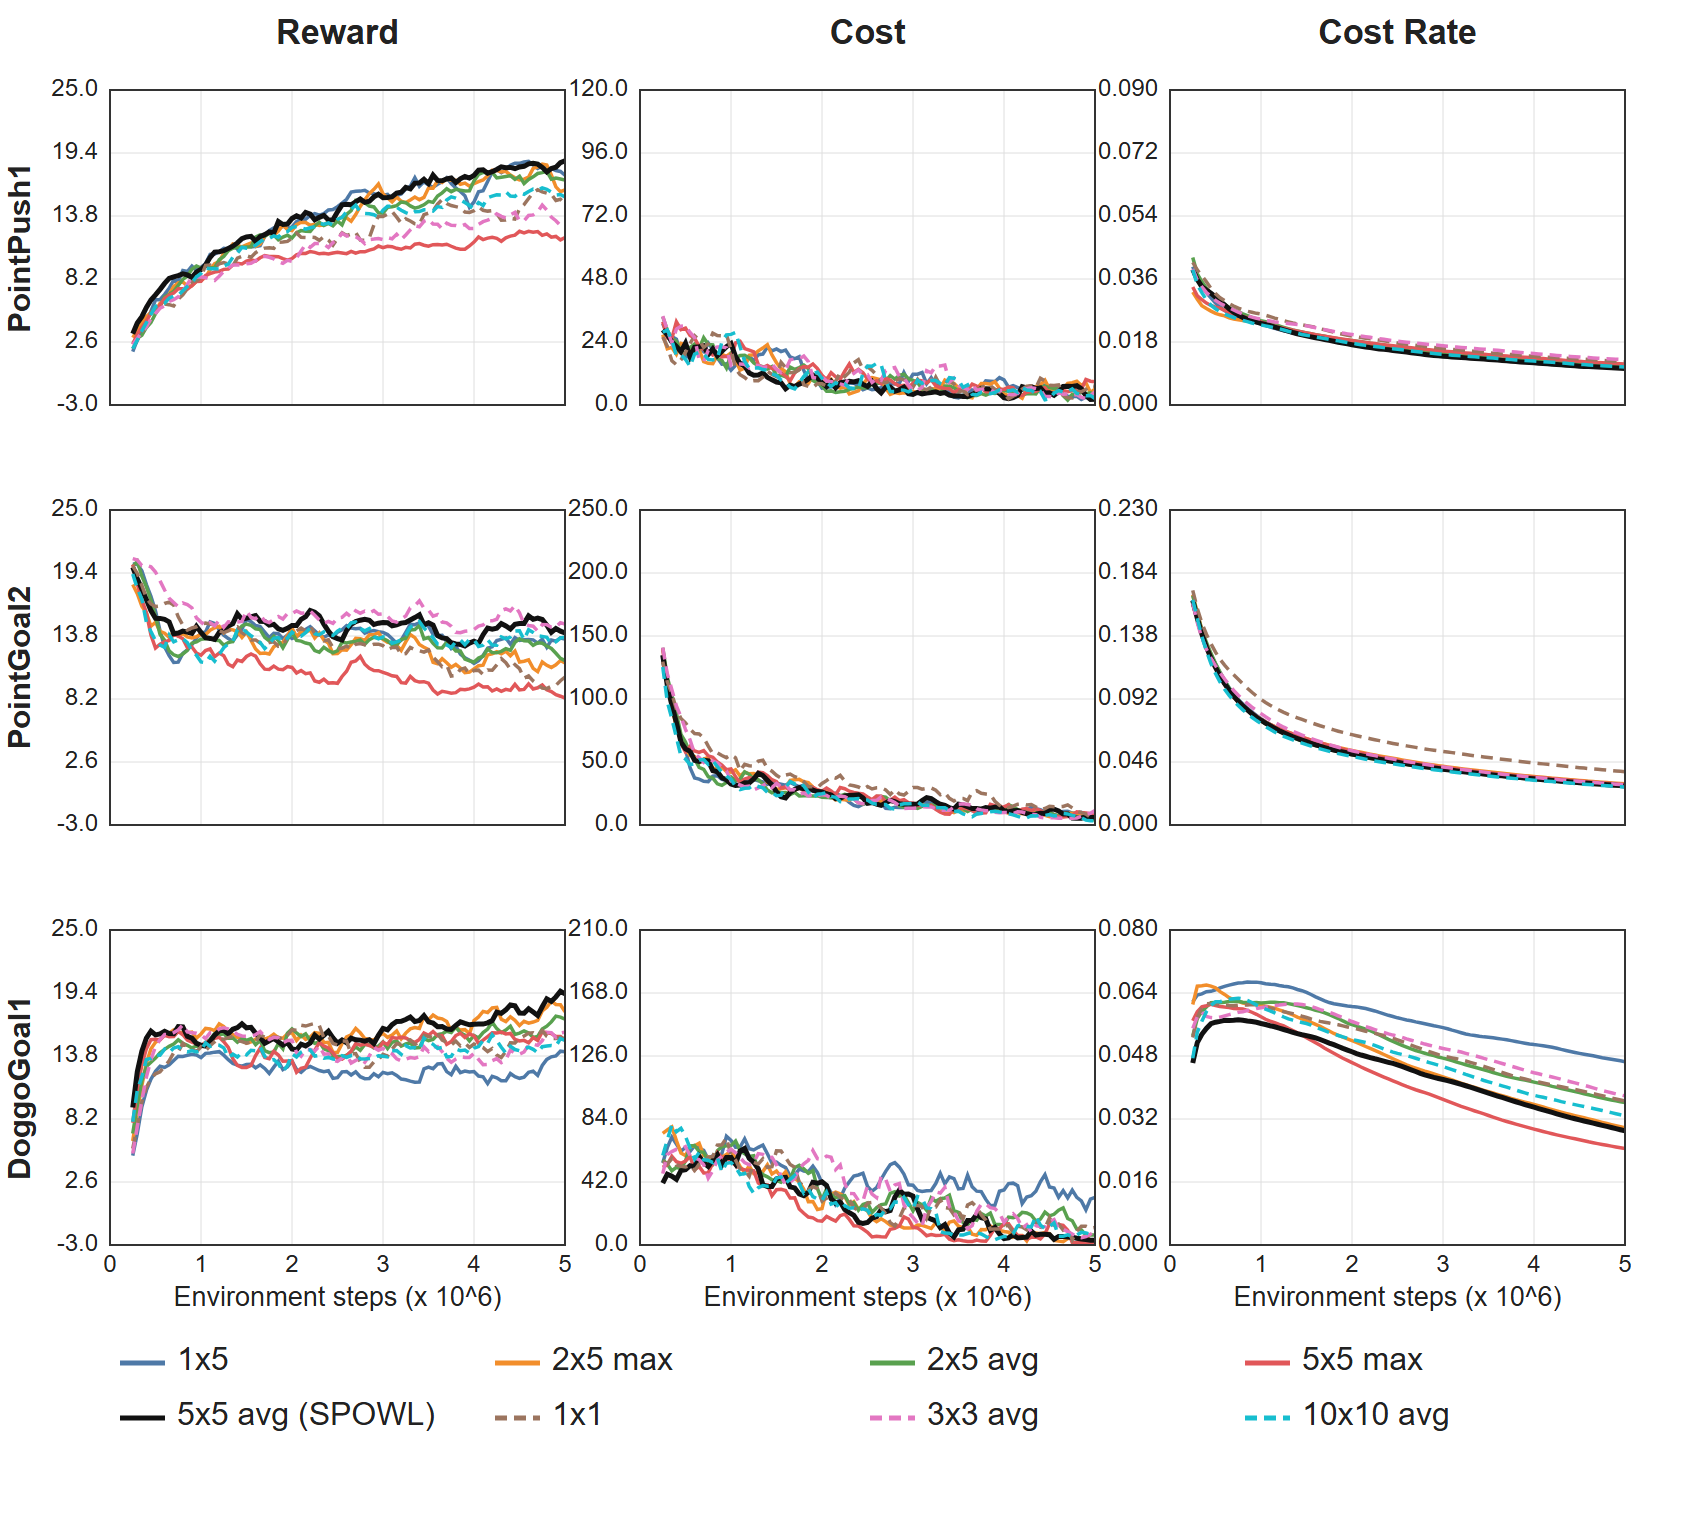
\includegraphics[width=\linewidth]{qa/qa_spowl_ensemble}
        \end{column}
    \end{columns}
\end{frame}

\qaQuestion{Котенко И.В.}{3}{%
    Предложенные методы принимают решения на основе текущего состояния среды и
    прогнозов модели мира. Как будут изменяться оценки безопасности при наличии
    ошибок или неполноты входных наблюдений? Возможно ли дополнить предложенные
    методы механизмом обнаружения таких ситуаций до выполнения потенциально
    опасного действия?}

\begin{frame}[noframenumbering]{Ответ на вопрос 3. Котенко И.В.}
    \small
    \begin{itemize}
        \item Модели, обученные без шума, при зашумлённых наблюдениях работают
              плохо. На модели мира ошибка влияет ещё сильнее, так как она
              предсказывает на несколько шагов вперёд.
        \item Стандартное решение --- аугментация: добавлять шум к входным
              данным (координатам и лидарам) при обучении.
        \item Для SG-Safe добавление гауссовского шума при обучении повышает
              успешность с $0.33$ до $0.80$ и снижает частоту столкновений с
              $0.27$ до $0.14$ при исполнении в зашумлённой среде.
    \end{itemize}
    \centering
    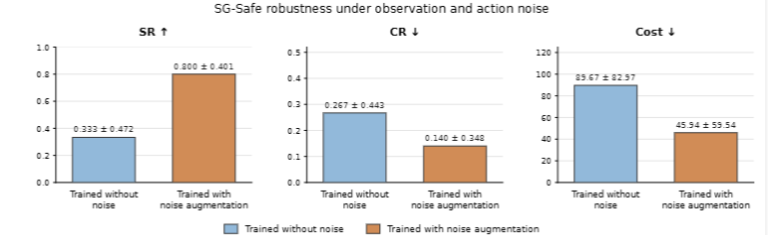
\includegraphics[width=0.9\linewidth]{qa/qa_sgsafe_noise}
\end{frame}

% ---------------------------------------------------------------------------
% Николенко С.И.
% ---------------------------------------------------------------------------

\begin{frame}[noframenumbering]{Вопрос 1. Николенко С.И.}
    \begin{block}{}
        \footnotesize
        Безопасность во время обучения. Тема диссертации --- безопасное
        исследование, то есть безопасность самого процесса обучения, и для её
        измерения в разделе 1.9 введена частота штрафов $\rho$. Однако в
        главе 4 для метода ITES приводятся преимущественно итоговые метрики
        после обучения (SR и Final Cost), которые не позволяют в полной мере
        оценить безопасность самого процесса исследования среды. Каковы
        значения $\rho$ для метода ITES на задачах с большим горизонтом ---
        SafeAntMazeCshape, SafeAntMazeWshape и SafePusher --- и как они
        соотносятся с показателями лучших базовых методов? Насколько полученные
        результаты подтверждают преимущество ITES именно с точки зрения
        безопасного исследования, а не только итоговой эффективности обученной
        стратегии? Кроме того, учитываются ли при расчёте $\rho$ первые
        30\,000 случайных шагов, используемых для предварительного обучения
        модели мира и модели штрафов?
    \end{block}
\end{frame}

\begin{frame}[noframenumbering,shrink=8]{Ответ на вопрос 1. Николенко С.И.}
    \small
    \begin{itemize}
        \item Важно не только безопасно исследовать, но и получить стратегию,
              которая решает задачу, поэтому оцениваются все три метрики ---
              $R$ (SR), $C$ и $\rho$ --- и во время обучения, и в конце.
        \item Наименьшее $\rho$ у метода, который плохо исследует среду, но
              безопасен (например, робот стоит на месте).
    \end{itemize}
    \centering
    \scriptsize
    \renewcommand{\arraystretch}{1.1}
    \begin{tabular}{l|ccc|ccc|ccc}
        \toprule
        & \multicolumn{3}{c|}{SafeAntMazeC} & \multicolumn{3}{c|}{SafeAntMazeW} & \multicolumn{3}{c}{SafePusher} \\
        Метод & $\rho\downarrow$ & SR$\uparrow$ & Cost & $\rho\downarrow$ & SR$\uparrow$ & Cost & $\rho\downarrow$ & SR$\uparrow$ & Cost \\
        \midrule
        \textbf{ITES}  & \textbf{0.078} & \textbf{0.88} & 15.2 & 0.179 & \textbf{0.35} & 183 & 0.422 & \textbf{0.42} & 12.8 \\
        SafeDreamer    & 0.099 & 0 & 13 & \textbf{0.170} & 0 & 216 & \textbf{0.034} & 0 & 6.7 \\
        CUP            & 0.107 & 0 & 6.8 & 0.229 & 0 & 103.5 & 0.437 & 0.01 & 46.1 \\
        FOCOPS         & 0.190 & 0 & 19.4 & 0.210 & 0 & 141 & 0.453 & 0 & 55.8 \\
        PPOLag         & 0.187 & 0.2 & 41.2 & --- & 0 & 105 & --- & 0 & 51.3 \\
        HRAC-LAG       & 0.182 & --- & --- & 0.351 & --- & --- & 0.217 & --- & --- \\
        \bottomrule
    \end{tabular}

    \vspace{0.4em}
    \raggedright
    \small
    \begin{itemize}
        \item На C-shape у ITES наименьшее $\rho$ при наибольшей SR; на
              W-shape $\rho$ на уровне SafeDreamer; на Pusher $\rho$ выше, но
              базовые методы задачу не решают (SR $\le 0.01$).
        \item Начальные шаги для обучения модели мира в $\rho$ ITES
              \textbf{не входят} (отдельный счётчик). Warm-up --- обычная
              практика для model-based методов; у SafeDreamer начальные шаги
              в $\rho$ входят.
    \end{itemize}
\end{frame}

\begin{frame}[noframenumbering]{Вопрос 2. Николенко С.И.}
    \begin{block}{}
        \footnotesize
        Глава 2, SPOWL. В таблице 2 SPOWL сравнивается с PPOLag, CPO и CVPO,
        которым разрешён бюджет 25 нарушений за эпизод, тогда как итоговый
        штраф самого SPOWL составляет от 0,3 до 5,4. Методы с бюджетом 25
        вправе тратить его и оптимизируют вознаграждение именно при этом
        ограничении, а у SPOWL явного бюджета нет: порог $d_c$ задаётся
        адаптивно, относительно оценок траекторий текущей стратегии. Как в
        таком случае задать для SPOWL уровень допустимых нарушений, требуемый
        пользователем, и что гарантирует его соблюдение? Второй вопрос касается
        самой оценки $Q_c$: целевое значение (2.9) строится по действию текущей
        стратегии, тогда как агент исполняет действия планировщика, а значит,
        терминальная оценка риска в (2.12) отвечает продолжению траектории
        стратегией, а не планировщиком. Насколько существенно это расхождение,
        когда планировщик заметно осторожнее (или смелее) стратегии?
    \end{block}
\end{frame}

\begin{frame}[noframenumbering,shrink=5]{Ответ на вопрос 2. Николенко С.И.}
    \small
    \begin{block}{Оценка безопасности плана: модель мира + терминальная оценка}
        \[
            J^{c,\mathrm{global}}_M(z_t, a_{t:t+H})
            = \underbrace{\sum_{i=0}^{H-1}\gamma_c^i\,\hat{c}_{t+i}}_{\text{план, модель мира}}
            + \underbrace{\gamma_c^H\,\hat{Q}^c_{\mathrm{agg}}(z_{t+H}, a_{t+H})}_{\text{продолжение стратегией},\ a_{t+H}\sim\pi}
        \]
    \end{block}
    \begin{itemize}
        \item \textbf{Бюджет.} PPOLag, CPO, CVPO не поддерживают адаптивное
              изменение бюджета, для этого нужен отдельный механизм; SPOWL
              решает эту проблему. При любом заданном бюджете выше
              достигаемого SPOWL будет его соблюдать: итоговый штраф уходит
              почти в ноль, и метод ведёт себя лучше базовых.
        \item \textbf{Согласованность оценки.} Да, оценка $Q_c$ относится к
              продолжению траектории стратегией, а не планировщиком.
              Но стратегия используется как базовый уровень: на каждом шаге
              SPOWL адаптивно выбирает действие планировщика или действие
              стратегии, поэтому в худшем случае агент ведёт себя как
              стратегия.
    \end{itemize}
\end{frame}

\begin{frame}[noframenumbering]{Вопрос 3. Николенко С.И.}
    \begin{block}{}
        \footnotesize
        Глава 3, SG-Safe. Бюджет $d = 3{,}0$ задан для дисконтированной оценки
        критика штрафов $Q_c(s, a)$ в (3.4), тогда как итоговая метрика MTSC
        --- недисконтированная сумма штрафов за эпизод, и на Point и Car она
        равна 20,7 (таблица 4). При этом в разделе 3.2.4 утверждается, что
        эпизодические штрафы остаются в рамках бюджета $d$. Как соотносятся эти
        величины и в каком смысле SG-Safe соблюдает ограничение? Заметим также,
        что по MTSC SG-Safe уступает SAC-LAG (13,7 против 12,8 в среднем по
        Safety Gym, 20,7 против 13,4 на Point; таблицы 4 и 6), так что выигрыш в
        доле успешных эпизодов покупается некоторым ростом штрафов. Это вполне
        возможный компромисс, но его стоило бы обсудить явно, например построив
        для обоих методов кривую <<успешность --- штраф>> для разных $d$. И
        уточняющий вопрос: совпадают ли 96 задач POLAMP, на которых проводится
        оценка, с задачами, на которых обучалась стратегия? Если да, то таблицы
        7--10 измеряют качество решения знакомых задач, а не обобщение на новые
        карты.
    \end{block}
\end{frame}

\begin{frame}[noframenumbering,shrink=10]{Ответ на вопрос 3. Николенко С.И.}
    \small
    \begin{columns}[T,onlytextwidth]
        \begin{column}{0.4\textwidth}
            \centering
            \scriptsize
            \begin{tabular}{llccc}
                \toprule
                & Метод & SR$\uparrow$ & CR$\downarrow$ & MTSC$\downarrow$ \\
                \midrule
                Point & SG-Safe & \textbf{0.93} & \textbf{0.02} & 20.7 \\
                      & SAC-LAG & 0.54 & 0.04 & \textbf{13.4} \\
                \midrule
                Avg.  & SG-Safe & \textbf{0.87} & \textbf{0.03} & 13.7 \\
                      & SAC-LAG & 0.40 & 0.05 & \textbf{12.8} \\
                \bottomrule
            \end{tabular}
        \end{column}
        \begin{column}{0.58\textwidth}
            \centering
            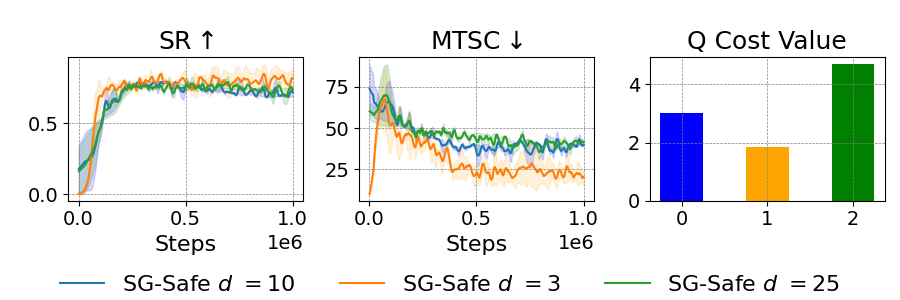
\includegraphics[width=\linewidth]{qa/qa_sgsafe_d_ablation}
        \end{column}
    \end{columns}
    \vspace{0.3em}
    \begin{itemize}
        \item $d$ --- гиперпараметр алгоритма для дисконтированного критика
              $Q_c$; бюджет задачи --- 25 нарушений за эпизод. MTSC SG-Safe
              ($20.7$ на Point и Car) остаётся в пределах бюджета задачи.
        \item $d$ выбирался по абляции (справа: $d \in \{3, 10, 25\}$);
              для SAC-LAG и других базовых методов использована реализация
              OmniSafe с уже подобранными гиперпараметрами.
        \item SG-Safe остаётся в рамках бюджета и лучше решает задачу, чем
              SAC-LAG, особенно на сложных задачах POLAMP (Level~2: SR $0.897$
              против $0$--$0.363$ у одноуровневых методов).
        \item \textbf{POLAMP:} карта фиксирована, но задачи на обучении и
              валидации различаются начальными и конечными состояниями.
              Сложность --- узкие коридоры относительно габаритов машины. На
              новых картах подход имеет потенциал при совместном
              использовании с классическим планировщиком.
    \end{itemize}
\end{frame}

\begin{frame}[noframenumbering]{Вопрос 4. Николенко С.И.}
    \begin{block}{}
        \footnotesize
        Глава 4, ITES. Низкоуровневая безопасность (4.9) оценивается моделью
        штрафов в одном случайно выбранном воображаемом состоянии, что даёт
        несмещённую оценку средней по траектории вероятности безопасности.
        Однако безопасность траектории в смысле ограничений --- это отсутствие
        нарушений на всей траектории, то есть произведение или минимум таких
        вероятностей, а не их среднее: траектория из девяти безопасных
        состояний и одного заведомо опасного имеет высокую среднюю
        безопасность. Почему выбрана именно средняя и не приводит ли это к
        тому, что стратегия просто <<разбавляет>> короткие опасные участки?
        Кроме того, на нижнем уровне безопасность входит в функцию потерь с
        фиксированным весом, а ограничение по Лагранжу накладывается только на
        верхнем уровне, так что бюджет $d$ формально контролируется лишь при
        выборе подцелей. Как подбирались веса безопасности на обоих уровнях и
        насколько результаты к ним чувствительны?
    \end{block}
\end{frame}

\begin{frame}[noframenumbering,shrink=8]{Ответ на вопрос 4. Николенко С.И.}
    \small
    \begin{itemize}
        \item В CMDP минимизируется не вероятность безопасности всей
              траектории, а \textbf{ожидаемый суммарный штраф}. При
              $n \sim U(\{1,\ldots,k-1\})$:
    \end{itemize}
    \vspace{-0.6em}
    \[
        \mathbb{E}_{n}\big[c(s_n)\big]
        = \frac{1}{k-1}\sum_{j=1}^{k-1} c(s_j)
        \quad\Longrightarrow\quad
        \arg\min\ \mathbb{E}_n\big[c(s_n)\big]
        = \arg\min \sum_{j=1}^{k-1} c(s_j).
    \]
    \vspace{-0.6em}
    \begin{itemize}
        \item Случайная точка вместо всего развёртывания:
              \begin{itemize}
                  \item модель мира --- простой ансамбль MLP (не RSSM, не
                        TD-MPC), ошибка накапливается по горизонту;
                  \item суммирование штрафов по всем воображаемым состояниям
                        приводит к взрыву градиентов (проверено
                        экспериментально);
                  \item со случайной точкой обучение стабильнее и быстрее, а
                        агент в среднем повышает безопасность всей траектории.
              \end{itemize}
        \item Бюджет $d$ контролируется на верхнем уровне --- это разделение
              ответственности: нижний уровень безопасно и эффективно достигает
              подцели, верхний, зная, как стратегия достигает подцелей,
              выбирает подцели так, чтобы уложиться в бюджет $d$.
        \item Веса $\beta^h_{safe}=800$, $\beta^l_{safe}=6$ подобраны по
              анализу чувствительности: при меньших весах растёт штраф, при
              больших агент становится чрезмерно консервативным и не решает
              задачу.
    \end{itemize}
\end{frame}

\qaQuestion{Николенко С.И.}{5}{%
    Глава 5, связь с остальной частью работы. Эксперименты на Caged CrafText
    диагностируют ровно ту проблему, которой посвящены главы 2--4: безопасные
    агенты перестают исследовать среду и застревают в первом найденном
    безопасном поведении. Почему на бенчмарке не оцениваются собственные
    методы автора --- SG-Safe, ITES или хотя бы оценка будущих накопленных
    штрафов в духе SPOWL? Такое сравнение было бы самой убедительной связью
    между частями диссертации.}

\begin{frame}[noframenumbering]{Ответ на вопрос 5. Николенко С.И.}
    \begin{itemize}
        \item Согласен, это хорошее направление для будущих исследований.
        \item Перенос SPOWL, SG-Safe и ITES на Caged CrafText --- отдельная
              нетривиальная задача:
              \begin{itemize}
                  \item как добавлять модальности: переводить изображения в
                        текстовое пространство или обучать совместный
                        энкодер;
                  \item как обрабатывать текстовые задачи на входе;
                  \item как адаптировать подцели ITES к целям в виде текста
                        или изображения.
              \end{itemize}
        \item Например, интеграция языковой модальности в Dreamer --- это
              отдельная работа и отдельный алгоритм (Dynalang).
    \end{itemize}
\end{frame}

% ---------------------------------------------------------------------------
% Мещеряков Р.В.
% ---------------------------------------------------------------------------

\qaQuestion{Мещеряков Р.В.}{1}{%
    В тексте диссертации следовало формализовать понятие безопасности, а также
    критерии, которые его определяют.}

\begin{frame}[noframenumbering]{Ответ на вопрос 1. Мещеряков Р.В.}
    \qaTodo
\end{frame}

\qaQuestion{Мещеряков Р.В.}{2}{%
    В методе ITES безопасность учитывается как при выборе промежуточных
    подцелей, так и при их достижении. Какой из этих двух механизмов вносит
    больший вклад в снижение числа нарушений безопасности? Можно ли оценить их
    влияние по отдельности?}

\begin{frame}[noframenumbering]{Ответ на вопрос 2. Мещеряков Р.В.}
    \begin{itemize}
        \item Да, влияние оценено по отдельности в абляционном исследовании
              ITES на SafeAntMaze: ITES, ITES без безопасности на нижнем
              уровне (w/o LLS) и ITES без безопасности на верхнем уровне
              (w/o HLS).
        \item Наибольший вклад даёт \textbf{безопасность подцелей}: если агент
              выбирает опасные подцели, он заезжает в опасную область, где
              нарушений много.
        \item Безопасность на нижнем уровне дополнительно снижает штраф и его
              разброс.
    \end{itemize}
    \centering
    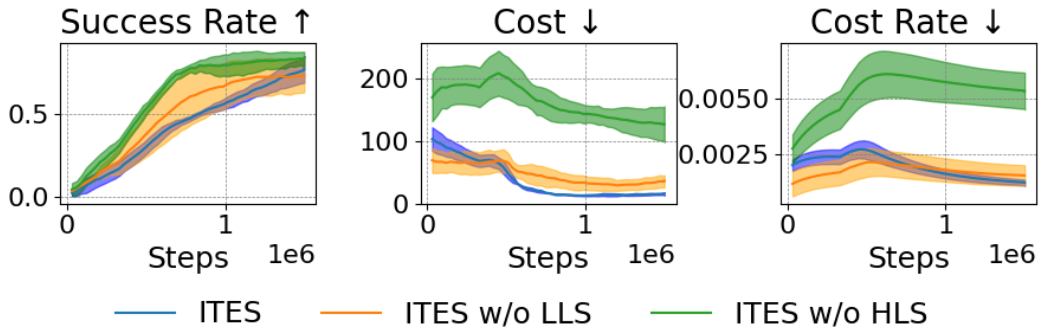
\includegraphics[width=0.85\linewidth]{Ablation_SafeAntMazeCshape_3}
\end{frame}

\qaQuestion{Мещеряков Р.В.}{3}{%
    В Caged CrafText агент должен соблюдать ограничения безопасности, заданные
    на естественном языке. Как можно экспериментально определить, связано ли
    нарушение ограничения с неправильным пониманием инструкции или с ошибкой
    при выборе действий?}

\begin{frame}[noframenumbering]{Ответ на вопрос 3. Мещеряков Р.В.}
    \qaTodo
\end{frame}

\qaQuestion{Мещеряков Р.В.}{4}{%
    В методе ITES верхнеуровневая стратегия выбирает промежуточные подцели с
    учётом ограничений безопасности, а низкоуровневая стратегия отвечает за их
    достижение. Каким образом агент должен действовать, если выбранная подцель
    оказывается недостижимой без нарушения ограничений безопасности? Какие
    механизмы могут использоваться для выбора альтернативной безопасной
    подцели?}

\begin{frame}[noframenumbering]{Ответ на вопрос 4. Мещеряков Р.В.}
    \qaTodo
\end{frame}

% ---------------------------------------------------------------------------
% Холодов Я.А.
% ---------------------------------------------------------------------------

\qaQuestion{Холодов Я.А.}{1}{%
    В методах SG-Safe и ITES верхний уровень формирует промежуточные подцели,
    которые затем достигаются низкоуровневой стратегией. Как выбор числа шагов
    между последовательными подцелями влияет на качество исследования и
    безопасность агента? Что происходит при слишком частом или, наоборот,
    слишком редком выборе новых подцелей?}

\begin{frame}[noframenumbering,shrink=5]{Ответ на вопрос 1. Холодов Я.А.}
    \small
    \begin{itemize}
        \item \textbf{SG-Safe:} подцели обучаются так, чтобы находиться
              посередине между текущим состоянием и целью.
        \item \textbf{ITES:} интервал $k$ фиксируется до обучения:
              $k=10$ для Safety Gym ($\approx$100 шагов на решение задачи),
              $k=20$ для SafeAntMaze ($\approx$300 шагов). Чем длиннее задача,
              тем больше можно взять $k$, но не слишком: подцель может
              устареть, если агенту нужен манёвр.
        \item Дополнительный эксперимент (SafeAntMazeC): малое $k$ ---
              безопаснее, но медленнее исследование; $k \ge 50$ --- агент не
              решает задачу.
    \end{itemize}
    \centering
    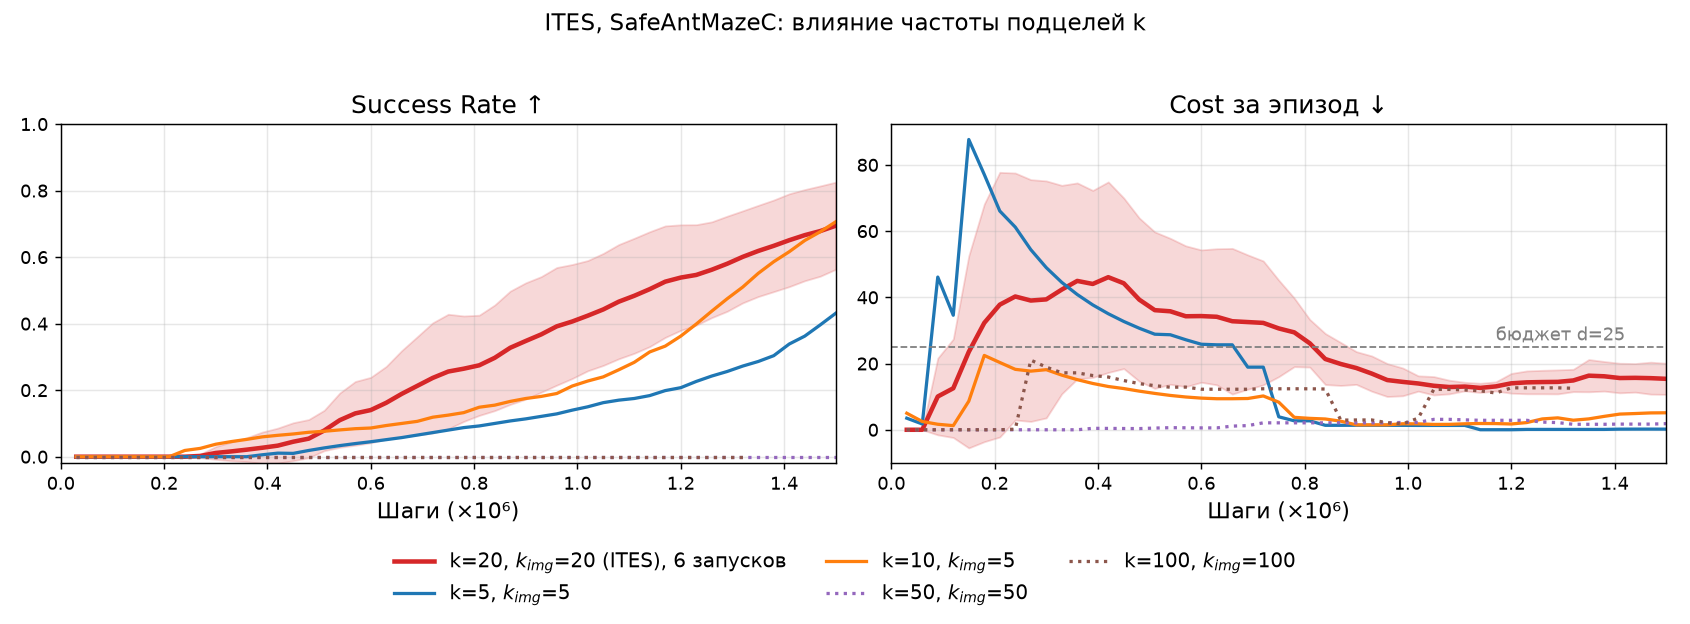
\includegraphics[width=0.92\linewidth]{qa/qa_ites_k_ablation}
\end{frame}

\qaQuestion{Холодов Я.А.}{2}{%
    В постановке безопасного обучения допустимый уровень нарушений задаётся
    бюджетом штрафов. Насколько результаты предложенных методов чувствительны к
    выбору этого бюджета? Можно ли использовать зависимость между успешностью
    выполнения задачи и накопленным штрафом для выбора разумного значения
    ограничения безопасности?}

\begin{frame}[noframenumbering,shrink=5]{Ответ на вопрос 2. Холодов Я.А.}
    \small
    \begin{itemize}
        \item Бюджет задаётся в начале обучения и влияет на разные компоненты:
              в SPOWL --- на консервативность фоновой стратегии (установлен
              минимальным), в ITES --- на генерацию подцелей, в SG-Safe --- на
              поведение низкоуровневой стратегии.
        \item Методы чувствительны к этому гиперпараметру, так как он задаёт
              суммарный уровень нарушений за эпизод; при $d=0$ методы, вероятно,
              не будут обучаться.
        \item Для SG-Safe и ITES $d$ подбирался по абляции (ниже --- SG-Safe).
        \item Правильнее уменьшать бюджет адаптивно до нуля в ходе обучения,
              по мере того как задача начинает решаться.
    \end{itemize}
    \centering
    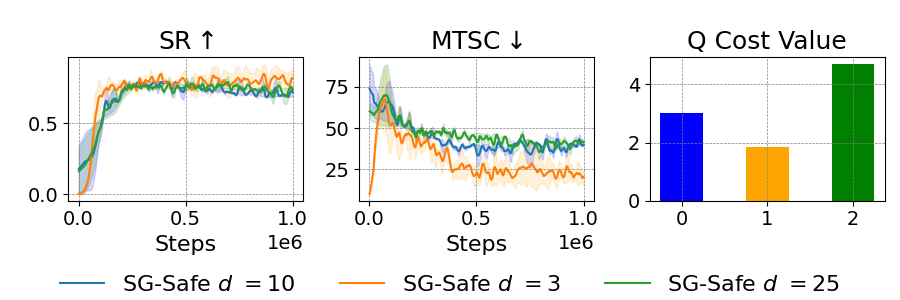
\includegraphics[width=0.85\linewidth]{qa/qa_sgsafe_d_ablation}
\end{frame}

\qaQuestion{Холодов Я.А.}{3}{%
    При обучении безопасной стратегии лишь небольшая часть переходов может
    содержать информацию о редких, но критичных нарушениях безопасности. Может
    ли выбор или приоритизация наиболее информативных эпизодов и переходов
    повысить эффективность обучения предложенных методов? По каким критериям
    целесообразно отбирать такой опыт?}

\begin{frame}[noframenumbering]{Ответ на вопрос 3. Холодов Я.А.}
    \begin{itemize}
        \item Да. По сути это проблема дисбаланса классов, как в классическом
              машинном обучении, но датасет собирается динамически. В первую
              очередь она влияет на обучение модели штрафов.
        \item В ITES эта проблема учтена: модель штрафов обучается на
              \textbf{сбалансированном буфере опыта}. Из каждой траектории в
              буфер добавляется поровну безопасных и опасных пар
              (подцель, состояние), поэтому батч в среднем содержит
              половину безопасных и половину опасных примеров.
        \item Критерий отбора --- наличие нарушения (класс примера); возможное
              развитие --- приоритизация по ошибке модели штрафов.
    \end{itemize}
\end{frame}
